\apendice{Especificación de Requisitos}

\section{Introducción}
En este anexo se pretenden indicar los distintos objetivos propuestos en el desarrollo de este proyecto. Así, como el conjunto de requisitos y sus especificaciones.

\section{Objetivos generales}
Los objetivos generales de este proyecto son los siguientes:

\begin{itemize}
	\item Realizar un estudio de las técnicas del estado del arte que solucionen el
reconocimiento automático de fitolitos con la mejor precisión y eficiencia posible. 
	\item Crear un sistema de etiquetación de fitolitos. Con el que podamos crear un conjunto de imágenes etiquetadas para llevar a cabo el sistema automático de reconocimiento de fitolitos.
	\item Crear un sistema que nos permita multiplicar en cantidad nuestro conjunto de imágenes. Debido al diminuto conjunto de imágenes que nos ha sido proporcionado.
	\item Crear un sistema capaz de reconocer fitolitos automáticamente en una imagen.
\end{itemize}

\section{Catálogo de requisitos}
Derivados de los objetivos anteriores, poseemos un conjunto de requisitos para el conjunto de aplicaciones resultantes de este proyecto.

\subsection{Requisitos funcionales}

\begin{itemize}
	\item \textbf{RF-1} Crear un sistema capaz de reconocer fitolitos automáticamente.
	\begin{itemize}
		\item \textbf{RF-1.1} Subir una nueva imagen y predecir donde se encuentran los distintos fitolitos.	\end{itemize}
	\item \textbf{RF-2} Crear una aplicación que permita el etiquetado de fitolitos. Con las siguientes funcionalidades:
	\begin{itemize}
		\item \textbf{RF-2.1} Escoger una imagen dentro de nuestro sistema operativo.
		\item \textbf{RF-2.2} Elegir entre los distintos tipos de fitolitos.
		\item \textbf{RF-2.3} Eliminar etiquetas realizadas sobre una imagen.
		\item \textbf{RF-2.5} Cargar una imagen previamente etiquetada junto a sus etiquetas.
		\item \textbf{RF-2.6} Guardar las coordenadas de las etiquetas y las imágenes de manera persistente.
		\item \textbf{RF-2.7} Notificar al usuario de los distintos eventos.
		\item \textbf{RF-2.8} Mostrar el tipo de fitolito etiquetado encima de cada etiqueta.
	\end{itemize}
	\item \textbf{RF-3} Crear una herramienta capaz de multiplicar el conjunto de imágenes etiquetadas de fitolitos mediante la aplicación de técnicas de \textit{data augmentation}.
	\begin{itemize}
		\item \textbf{RF-3.1} Elegir el número de imágenes resultantes.
		\item \textbf{RF-3.2} Reescalarlas.		
		\item \textbf{RF-3.3} Rotarlas.
		\item \textbf{RF-3.4} Espejarlas.
		\item \textbf{RF-3.5} Aplicarlas ruidos.
		\item \textbf{RF-3.6} Aplicarlas filtros de oscurecimiento y aclaramiento.
		\item \textbf{RF-3.7} Aplicarlas aleatoriamente las distintas modificaciones anteriores, permitiendo el mayor número de combinaciones posible.
	\end{itemize}
\end{itemize}

\subsection{Requisitos no funcionales}

\begin{itemize}
	\item \textbf{RNF-1} Facilidad de uso: las herramientas diseñadas para el usuario final deben ser intuitivas y fáciles de utilizar con una mínima formación.
\end{itemize}

\section{Especificación de requisitos}

La especificación de requisitos será explicada mediante diagramas de casos de uso en notación UML\footnote{UML, según sus siglas Lenguaje de Modelado Unificado, es una notación comúnmente utilizada para representar y documentar un sistema con una mayor abstracción~\cite{wiki:uml}.} y una tabla por cada caso de uso, la cual los explica en mayor detalle.

\subsection{Diagramas de casos de uso}

\begin{figure}
\centering
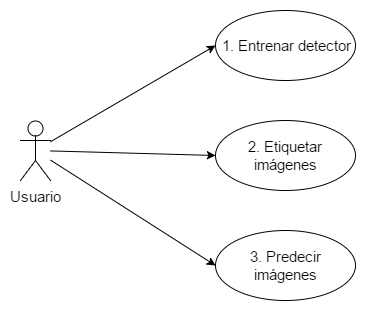
\includegraphics[width=0.5\textwidth]{dia_uc}
\caption{Diagrama general de casos de uso.}
\label{fig:B.1}
\end{figure}

\begin{figure}
\centering
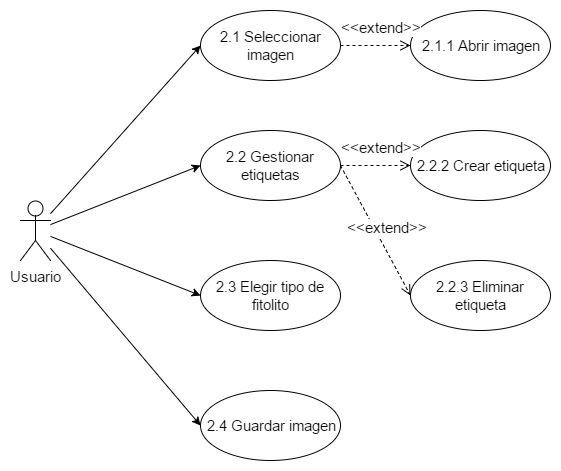
\includegraphics[width=0.9\textwidth]{dia_uc1}
\caption[Diagrama extendido]{Diagrama extendido del segundo caso de uso del anterior.}
\label{fig:B.2}
\end{figure}




\tablaSmallSinColores{Caso de uso 1: Entrenar detector}{p{3cm} p{.75cm} p{9.5cm}}{tablaUC1}{
  \multicolumn{3}{l}{Caso de uso 1:  Entrenar detector} \\
 }
 {
  Descripción                            & \multicolumn{2}{p{10.25cm}}{Permite al usuario entrenar el detector automático de fitolitos.} \\\hline
  \multirow{2}{3.5cm}{Requisitos}  & \multicolumn{2}{p{10.25cm}}{RF-1} 
  \\\cline{2-3}
                                         & \multicolumn{2}{p{10.25cm}}{RF-1.1}
                                         \\\hline
  Precondiciones                         &  \multicolumn{2}{p{10.25cm}}{Tener instalado \textit{darkflow}.}   \\\hline
  \multirow{2}{3.5cm}{Secuencia normal}  & Paso & Acción \\\cline{2-3}
                                         & 1    & El usuario lanza el comando de entrenamiento.
  \\\cline{2-3}
                                         & 2    & Se carga el modelo.
  \\\cline{2-3}
                                         & 3    & Se cargan los pesos del modelo.
    \\\cline{2-3}
                                         & 4    & Se convierten las coordenadas de las etiquetas.                                           	\\\cline{2-3}
                                         & 5    & Se comienza el entrenamiento. 
                                         \\\hline
  Postcondiciones                        & \multicolumn{2}{p{10.25cm}}{Se guardan unos ficheros con los pesos resultantes del entrenamiento.} \\\hline
  Excepciones                        & \multicolumn{2}{p{10.25cm}}{La elección de opciones no compatibles entre sí.}\\\hline
  Importancia                            & Alta \\\hline
  Urgencia                               & Media \\
}





\tablaSmallSinColores{Caso de uso 2: Etiquetar imágenes}{p{3cm} p{.75cm} p{9.5cm}}{tablaUC2}{
  \multicolumn{3}{l}{Caso de uso 2:  Etiquetar imágenes} \\
 }
 {
  Descripción                            & \multicolumn{2}{p{10.25cm}}{Permite al usuario identificar los múltiples tipos de fitolitos.} \\\hline
  \multirow{2}{3.5cm}{Requisitos}  &\multicolumn{2}{p{10.25cm}}{RF-2} \\\cline{2-3}
                                         & \multicolumn{2}{p{10.25cm}}{RF-2.1} \\\cline{2-3}
                                         & \multicolumn{2}{p{10.25cm}}{RF-2.2}  \\\cline{2-3}
                                         & \multicolumn{2}{p{10.25cm}}{RF-2.3}  \\\cline{2-3}
                                         & \multicolumn{2}{p{10.25cm}}{RF-2.4}  \\\cline{2-3}
                                         & \multicolumn{2}{p{10.25cm}}{RF-2.5}  \\\cline{2-3}
                                         & \multicolumn{2}{p{10.25cm}}{RF-2.6}  \\\cline{2-3}
                                         & \multicolumn{2}{p{10.25cm}}{RF-2.7}  \\\cline{2-3}
                                         & \multicolumn{2}{p{10.25cm}}{RF-2.8}
                                         \\\hline
  Precondiciones                         &    \multicolumn{2}{p{10.25cm}}{Ejecutar el \textit{Jupyter Notebook}.}    \\\hline
  \multirow{2}{3.5cm}{Secuencia normal}  & Paso & Acción \\\cline{2-3}
                                         & 1    & El usuario selecciona una imagen.
  \\\cline{2-3}
                                         & 2    & La imagen se carga.
  \\\cline{2-3}
                                         & 3    & El usuario etiqueta los fitolitos.
    \\\cline{2-3}
                                         & 4    & El usuario pulsa en el botón guardar.                                           	\\\cline{2-3}
                                         & 5    & Se guardan las imágenes y coordenadas. 
                                         \\\hline
  Postcondiciones                        & \multicolumn{2}{p{10.25cm}}{Se guardan los ficheros que almacenan las coordenadas de las etiquetas y las imágenes.} \\\hline
  Excepciones                        & \multicolumn{2}{p{10.25cm}}{Tratar de cargar un documento distinto a una imagen.}\\\hline
  Importancia                            & Alta \\\hline
  Urgencia                               & Alta \\
}




\tablaSmallSinColores{Caso de uso 3: Predecir imágenes}{p{3cm} p{.75cm} p{9.5cm}}{tablaUC3}{
  \multicolumn{3}{l}{Caso de uso 3:  Predecir imágenes} \\
 }
 {
  Descripción                            & \multicolumn{2}{p{10.25cm}}{Permite al usuario identificar los fitolitos en una imagen.} \\\hline
  \multirow{2}{3.5cm}{Requisitos}  &\multicolumn{2}{p{10.25cm}}{RF-1} \\\cline{2-3}
                                         & \multicolumn{2}{p{10.25cm}}{RF-1.1} \\\hline
  Precondiciones                         &    \multicolumn{2}{p{10.25cm}}{}    \\\hline
  \multirow{2}{3.5cm}{Secuencia normal}  & Paso & Acción \\\cline{2-3}
                                         & 1    & El usuario escoge una imagen.
  \\\cline{2-3}
                                         & 2    & El usuario pulsa en el botón para predecir una nueva imagen. 	\\\cline{2-3}
                                         & 5    & Se predice la imagen. 
    \\\cline{2-3}
                                         & 6    & Se muestran los resultados. 
                                         \\\hline
  Postcondiciones                        & \multicolumn{2}{p{10.25cm}}{} \\\hline
  Excepciones                        & \multicolumn{2}{p{10.25cm}}{Tratar de cargar un documento distinto a una imagen.
  Escoger erróneamente las configuraciones.}\\\hline
  Importancia                            & Alta \\\hline
  Urgencia                               & Alta \\
}




\tablaSmallSinColores{Caso de uso 2.1: Seleccionar imagen}{p{3cm} p{.75cm} p{9.5cm}}{tablaUC1.1}{
  \multicolumn{3}{l}{Caso de uso 2.1:  Seleccionar imagen} \\
 }
 {
  Descripción                            & \multicolumn{2}{p{10.25cm}}{El usuario puede seleccionar una imagen desde su sistema operativo. La cual se carga, muestra y finalmente se le permite etiquetarla.} \\\hline
  \multirow{2}{3.5cm}{Requisitos}  &\multicolumn{2}{p{10.25cm}}{RF-2} \\\cline{2-3}
                                         & \multicolumn{2}{p{10.25cm}}{RF-2.1} \\\cline{2-3}
                                         & \multicolumn{2}{p{10.25cm}}{RF-2.5}  \\\cline{2-3}
                                         & \multicolumn{2}{p{10.25cm}}{RF-2.7}  \\\cline{2-3}
                                         & \multicolumn{2}{p{10.25cm}}{RF-2.8}
                                         \\\hline
  Precondiciones                         &   Ninguna   & 
  \\\hline
  \multirow{2}{3.5cm}{Secuencia normal}  & Paso & Acción \\\cline{2-3}
                                         & 1    & El usuario pulsa el botón de subida de imágenes. 
  \\\cline{2-3}
                                         & 2    & El usuario selecciona una imagen.
  \\\cline{2-3}
                                         & 3    & El usuario pulsa el botón de abrir imagen.
    \\\cline{2-3}
                                         & 4    & Se carga la nueva imagen.                                           	\\\cline{2-3}
                                         & 5    & Se notifica al usuario. 
                                         \\\hline
  Postcondiciones                        & \multicolumn{2}{p{10.25cm}}{La imagen se muestra por pantalla.} \\\hline
  Excepciones                        & \multicolumn{2}{p{10.25cm}}{No se ha seleccionado una imagen, sino un documento u otro tipo de fichero.}\\\hline
  Importancia                            & Alta \\\hline
  Urgencia                               & Alta \\\hline
  Comentarios                            & & \\
}




\tablaSmallSinColores{Caso de uso 2.2: Gestionar etiquetas}{p{3cm} p{.75cm} p{9.5cm}}{tablaUC2.2}{
  \multicolumn{3}{l}{Caso de uso 2.2:  Gestionar etiquetas} \\
 }
 {
  Descripción                            & \multicolumn{2}{p{10.25cm}}{El usuario podrá crear y eliminar etiquetas.} \\\hline
  \multirow{2}{3.5cm}{Requisitos}  & \multicolumn{2}{p{10.25cm}}{RF-2}  \\\cline{2-3}  & \multicolumn{2}{p{10.25cm}}{RF-2.3}  \\\cline{2-3}  & \multicolumn{2}{p{10.25cm}}{RF-2.8}  \\\hline
  Precondiciones                         &   Ninguna   & \\\hline
  \multirow{2}{3.5cm}{Secuencia normal}  & Paso & Acción \\\cline{2-3}
                                         & 1    & Si el usuario clica sobre una <<x>>. 
  \\\cline{2-3}
                                         & 1.2    & Se borra etiqueta.  
  \\\cline{2-3}
                                         & 2    & Sino:
  \\\cline{2-3}
                                         & 2.2    & Se crea una etiqueta.  \\\hline
  Postcondiciones                        & \multicolumn{2}{p{10.25cm}}{ Se cambia el estado de las etiquetas.} \\\hline
  Excepciones                        & \multicolumn{2}{p{10.25cm}}{Ninguna.}\\\hline
  Importancia                            & Alta \\\hline
  Urgencia                               & Alta \\\hline
  Comentarios                            & \multicolumn{2}{p{10.25cm}}{Se permite crear etiquetas fuera de la imagen y sin haber cargado una imagen. Pero estas no se guardarán.} \\
}





\tablaSmallSinColores{Caso de uso 2.3: Elegir tipo de fitolito}{p{3cm} p{.75cm} p{9.5cm}}{tablaUC2.3}{
  \multicolumn{3}{l}{Caso de uso 2.3:  Elegir tipo de fitolito} \\
 }
 {
  Descripción                            & \multicolumn{2}{p{10.25cm}}{El usuario puede elegir entre los distintos tipos de fitolito antes de realizar una etiqueta.} \\\hline
  \multirow{2}{3.5cm}{Requisitos}  & \multicolumn{2}{p{10.25cm}}{RF-2} \\\cline{2-3}  & \multicolumn{2}{p{10.25cm}}{RF-2.2}  \\\cline{2-3}  & \multicolumn{2}{p{10.25cm}}{RF-2.6} \\\cline{2-3}  & \multicolumn{2}{p{10.25cm}}{RF-2.8}  \\\hline
  Precondiciones                         &   Ninguna   & \\\hline
  \multirow{2}{3.5cm}{Secuencia normal}  & Paso & Acción \\\cline{2-3}
                                         & 1    & El usuario pulsa sobre el botón del tipo de fitolito que desee. 
  \\\cline{2-3}
                                         & 2    & Se realiza un cambio en las distintas variables que incorporan información dependiente del tipo de fitolito. Como el directorio en el que guardar el recorte.
                                         \\\hline
  Postcondiciones                        & \multicolumn{2}{p{10.25cm}}{Cambios en las variables dependientes del contexto de este.} \\\hline
  Excepciones                        & \multicolumn{2}{p{10.25cm}}{Ninguna.}\\\hline
  Importancia                            & Media \\\hline
  Urgencia                               & Media \\\hline
  Comentarios                            & \multicolumn{2}{p{10.25cm}}{La selección del tipo de fitolito permite distinguir donde o como guardar la información. Por lo tanto, es fundamental.} \\
}




\tablaSmallSinColores{Caso de uso 2.4: Guardar imagen}{p{3cm} p{.75cm} p{9.5cm}}{tablaUC2.4}{
  \multicolumn{3}{l}{Caso de uso 2.4:  Guardar imagen} \\
 }
 {
  Descripción                            & \multicolumn{2}{p{10.25cm}}{El usuario puede guardar las  coordenadas y la imagen que haya sido etiquetada.} \\\hline
  Precondiciones                         &   Ninguna   & \\\hline
  \multirow{2}{3.5cm}{Secuencia normal}  & Paso & Acción \\\cline{2-3}
                                         & 1    & El usuario pulsa en el boton guardar de la imagen. 
  \\\cline{2-3}
                                         & 2    & Se guardan las coordenadas y la imagen de manera persistente. \\\hline
  Postcondiciones                        & \multicolumn{2}{p{10.25cm}}{La imagen y coordenadas se almacenan localmente.} \\\hline
  Excepciones                        & \multicolumn{2}{p{10.25cm}}{Ninguna.}\\\hline
  Importancia                            & Alta \\\hline
  Urgencia                               & Alta \\\hline
  Comentarios                            & \multicolumn{2}{p{10.25cm}}{} \\
}




\tablaSmallSinColores{Caso de uso 2.1.1: Abrir imagen}{p{3cm} p{.75cm} p{9.5cm}}{tablaUC2.1.1}{
  \multicolumn{3}{l}{Caso de uso 2.1.1:  Abrir imagen} \\
 }
 {
  Descripción                            & \multicolumn{2}{p{10.25cm}}{El usuario puede abrir una imagen.} \\\hline
  Precondiciones                         &   \multicolumn{2}{p{10.25cm}}{El usuario ha seleccionado una imagen.}
  \\\hline
    \multirow{2}{3.5cm}{Requisitos}  &\multicolumn{2}{p{10.25cm}}{RF-2} \\\cline{2-3}
                                         & \multicolumn{2}{p{10.25cm}}{RF-2.1} \\\hline
  \multirow{2}{3.5cm}{Secuencia normal}  & Paso & Acción \\\cline{2-3}
                                         & 1    & El usuario selecciona la imagen 
  \\\cline{2-3}
                                         & 2    & Se carga la información de la imagen.
  \\\cline{2-3}
                                         & 3    & Se guarda persistentemente.  \\\hline
  Postcondiciones                        & \multicolumn{2}{p{10.25cm}}{Se guarda la imagen en el almacenamiento.} \\\hline
  Excepciones                        & \multicolumn{2}{p{10.25cm}}{No se ha seleccionado una imagen, sino un documento u otro tipo de fichero.}\\\hline
  Importancia                            & Alta \\\hline
  Urgencia                               & Alta \\\hline
  Comentarios                            & & \\
}



\tablaSmallSinColores{Caso de uso 2.2.2: Crear Etiqueta}{p{3cm} p{.75cm} p{9.5cm}}{tablaUC2.2.2}{
  \multicolumn{3}{l}{Caso de uso 2.2.2:  Crear Etiqueta} \\
 }
 {
  Descripción                            & \multicolumn{2}{p{10.25cm}}{El usuario puede etiquetar los distintos tipos de fitolitos en la imagen.} \\\hline
  Precondiciones                         &   Ninguna   & \\\hline
  \multirow{2}{3.5cm}{Secuencia normal}  & Paso & Acción \\\cline{2-3}
                                         & 1    & El usuario pulsa un click sobre la imagen. 
  \\\cline{2-3}
                                         & 2    & El usuario mueve el ratón por la imagen.
  \\\cline{2-3}
                                         & 3    & El usuario vuelve a pulsar un click para realizar una etiqueta.
                                         \\\cline{2-3}
                                         & 4    & Se escribe por encima de la etiqueta el tipo de fitolito.
                                         \\\cline{2-3}
                                         & 5    & Se añade una cruz que permite la eliminación de la etiqueta.
                                         \\\hline
  Postcondiciones                        & \multicolumn{2}{p{10.25cm}}{La etiqueta se define encima de la imagen.} \\\hline
  Excepciones                        & \multicolumn{2}{p{10.25cm}}{Ninguna.}\\\hline
  Importancia                            & Alta \\\hline
  Urgencia                               & Alta \\\hline
  Comentarios                            & \multicolumn{2}{p{10.25cm}}{Se permite crear etiquetas fuera de la imagen y sin haber cargado una imagen. Pero estas no se guardarán.} \\
}


\tablaSmallSinColores{Caso de uso 2.2.3: Eliminar Etiqueta}{p{3cm} p{.75cm} p{9.5cm}}{tablaUC2.2.3}{
  \multicolumn{3}{l}{Caso de uso 2.2.3:  Eliminar Etiqueta} \\
 }
 {
  Descripción                            & \multicolumn{2}{p{10.25cm}}{El usuario puede eliminar las distintas etiquetas realizadas en una imagen.} \\\hline
  Precondiciones                         &   Ninguna   & \\\hline
  \multirow{2}{3.5cm}{Secuencia normal}  & Paso & Acción \\\cline{2-3}
                                         & 1    & El usuario pulsa un click sobre <<x>> de una etiqueta. 
  \\\cline{2-3}
                                         & 2    & Se elimina la representación de esa etiqueta.
  \\\cline{2-3}
                                         & 3    & Se eliminan las coordenadas asociadas a la etiqueta.  \\\hline
  Postcondiciones                        & \multicolumn{2}{p{10.25cm}}{La etiqueta se elimina visual e internamente.} \\\hline
  Excepciones                        & \multicolumn{2}{p{10.25cm}}{Ninguna.}\\\hline
  Importancia                            & Baja \\\hline
  Urgencia                               & Baja \\\hline
  Comentarios                            & \multicolumn{2}{p{10.25cm}}{} \\
}